\documentclass{article}
\usepackage[utf8]{inputenc}

\title{EE2703 Applied Programming Lab \\ Assignment 5}
\author{
  \textbf{Name}: Neham Hitesh Jain\\
  \textbf{Roll Number}: EE19B084
}\date{March 26, 2021}

\usepackage{listings}
\usepackage{natbib}
\usepackage{amsmath}
\usepackage{color}
\usepackage{graphicx}
\definecolor{dkgreen}{rgb}{0,0.6,0}
\definecolor{gray}{rgb}{0.5,0.5,0.5}
\definecolor{mauve}{rgb}{0.58,0,0.82}

\lstset{frame=tb,
  language=Python,
  aboveskip=3mm,
  belowskip=3mm,
  showstringspaces=false,
  columns=flexible,
  basicstyle={\small\ttfamily},
  numbers=none,
  numberstyle=\tiny\color{gray},
  keywordstyle=\color{blue},
  commentstyle=\color{dkgreen},
  stringstyle=\color{mauve},
  breaklines=true,
  breakatwhitespace=true,
  tabsize=3
}

\begin{document}

\maketitle
\newpage

\section{Abstract}
The aim is to find the solution to potential on a plate by solving the Laplace equation
In this assignment, we attempt to find the solution to potential on a plate by solving the Laplace equation,
 analyze the current flow across the cross-section of a circular wire (resistor) and, consequentially, the temperature
distribution of the cross section of the wire.


\section{Introduction}
A  cylindrical wire is soldered to the middle of a copper plate of dimension 1cm by 1cm. Voltage of the wire is held at 1 Volt.  
Bottom side of the plate is grounded, while the remaining are kept floating.
\newline \newline
We make use of the 3 fundamental equation to solve this problem:
\newline
\begin{equation}
    \nabla \cdot \vec{j} = - \frac{\partial\rho}{\partial t}
\end{equation}
\begin{equation}
    \vec{j} = \sigma\vec{E}
\end{equation}
\begin{equation}
    \vec{E} = -\nabla\phi
\end{equation}
From the above equations:
\begin{equation}
    \nabla^2 \phi =  \frac{1}{\rho}\frac{\partial\rho}{\partial t}
\end{equation}
Now, For DC Currents, RHS of equation (3) is 0. Hence:
\begin{equation}
    \label{eqn(5)}
    \nabla^2 \phi =  0
\end{equation}
Laplace's equation in 2-dimensions can  be written in Cartesian coordinates as 
\begin{equation}
    \label{eqn(6)}
    \frac{\partial^2 \phi}{\partial x^2} + \frac{\partial^2 \phi}{\partial y^2} = 0
\end{equation}

To define the plate dimensions and wire size we take inputs from the user and use the following
code to setup the grid.
\begin{lstlisting}

def create_grid(x,y,radius):    
    ''' Creating grid of coordinates of the plate and initialising phi'''
    phi_initial=np.zeros((y,x))
    xx = np.linspace(-0.5,0.5,y)
    yy = np.linspace(-0.5,0.5,x)
    Y_coords,X_coords = np.meshgrid(yy,xx)
    wire_loc = np.where((X_coords**2 + Y_coords**2) < (radius/x)**2)
    phi_initial[wire_loc]=1
    return X_coords,Y_coords,phi_initial,wire_loc

\end{lstlisting}


\section{Finding Potential Matrix}
\subsection{ Initializing Potential Matrix}
We represent the grid of data points of size Nx x Ny using a matrix of same size. 
We initialize it with 0 and then we find the points lying within the wire and initialize them to 1. We then plot its contour plot.
\begin{lstlisting}
def contour_plot(self,x,y,phi,wire_loc,cmap=plt.get_cmap('hot')):
    axes=self.fig.add_subplot(111)
    t=axes.contourf(y,x[::-1],phi,cmap=cmap)
    axes.plot(x[:,0][wire_loc[0]],y[0,:][wire_loc[1]],'ro')
    axes.grid()
    self.fig.colorbar(t)
    self.general_funcs(axes)
\end{lstlisting}
\begin{figure}[h!]
\centering
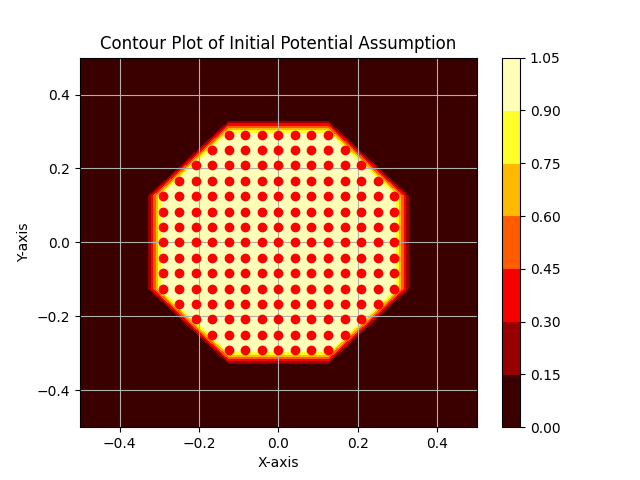
\includegraphics[scale=0.6]{plots/Contour Plot of Initial Potential Assumption.png}
\caption{Initial Potential}
\label{fig:initial Potential}
\end{figure}

\subsection{Iterating and Updating potential}
\subsubsection{Updating matrix}
We use the constraint given by Equation 6 to update the values of potential. However the equation is in differential form which we convert to discrete form 
An approximate solution for the above equation for a 2-dimensional grid of points would be 
\begin{equation*}
\phi_{i,j} = \frac{\phi_{i,j-1}+\phi_{i-1,j}+\phi_{i+1,j}+\phi_{i,j+1}}{4} 
\end{equation*}
ie. the solution at any point is a sum of values at neighbouring points. The algorithm implemented makes 
use of the above equation to update $\phi$  over many iterations till it converges within an acceptable error.

Also, we find the error between two iterations by taking the maximum of the absolute differences between corresponding 
data entries of the old and updated voltage matrices and store it in error array.

\begin{lstlisting}
for i in range(epochs):
    oldphi=phi.copy()   #Need a proper copy not a view
    phi[1:-1,1:-1]=0.25*(phi[1:-1,0:-2]+ phi[1:-1,2:]+phi[0:-2,1:-1]+ phi[2:,1:-1])    #Laplace Equation
    phi=boundary_conditions(phi,wire_loc)
    errors[i]=(abs(phi-oldphi)).max()   #Calculate errors.
\end{lstlisting}

\subsubsection{Applying Boundary Conditions}
As no currents flows out of the top,left,right boundary the gradient at the potential at boundary must be 0. 
Also the bottom boundary is grounded. We apply this boundary condition after every iteration
\begin{lstlisting}
def boundary_conditions(phi,wire_loc):
    ''' Function to enforce appropriate boundary conditions''' 

    phi[1:-1,0] = phi[1:-1,1]   #Left side boundary condition
    phi[0,1:-1] = phi[1,1:-1]   #Top side
    phi[1:-1,-1] = phi[1:-1,-2] #Right side boundary condition
    phi[-1,1:-1] = 0            #Bottom part of plate is kept grounded
    phi[wire_loc] = 1.0         #Wire locations are at 1V
    return phi
\end{lstlisting}

\section{Error Analysis}
\subsection{Calculating error and plotting}

We first plot the error (ie. maximum absolute difference between old $\phi$ and $\phi$ at every step)
with number of iterations on a linear scale and see that it changes very slowly after a while,
hence we also analyse the plots in a semi-log scale and log-log scale.

\begin{figure}[h!]
    \centering
    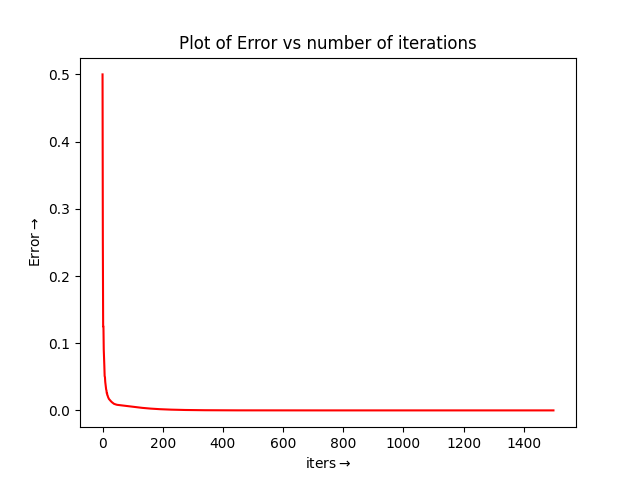
\includegraphics[scale=0.6]{plots/Plot of Error vs number of iterations.png}
    \caption{Error plot in linear scale}
    \label{fig2}
\end{figure}

\subsection{Fitting the error to an exponential}

We see that the errors decreases pretty slowly with iterations and thus we plot them on semilogy and loglog plots.

We also observe that the error decreases in exponential form and thus we fit the error on a exponential and also plot that alongside the original error plot. However the exponential decay is only after around 500 iterations. Thus we plot two fits, one considering the error values of all the iterations and other with only after 500 iterations.

\begin{lstlisting}

def fit_exp(x,A,B):
    ''' Function to obtain an exponential '''
    return A*np.exp(B*x)

def error_fit(x,y):
    ''' Evaluates the parameters of an exponent. x is the data vector, y is the vector of true values ''' 
    logy=np.log(y)
    xvec=np.zeros((len(x),2))
    xvec[:,0]=x
    xvec[:,1]=1
    B,logA=np.linalg.lstsq(xvec, np.transpose(logy),rcond=None)[0]
    return (np.exp(logA),B)


\end{lstlisting}
\begin{figure}[h!]
\centering
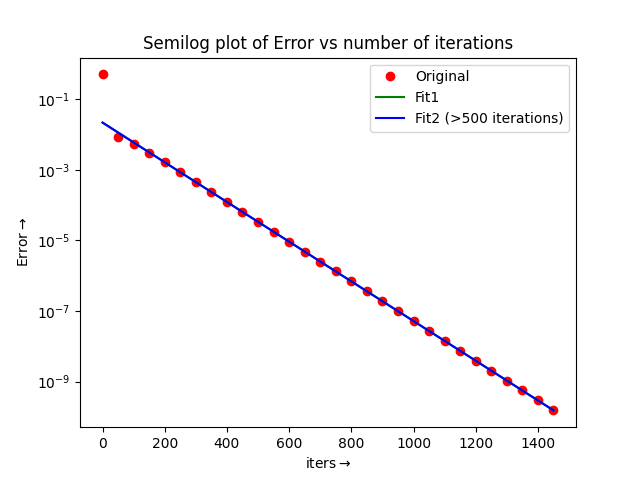
\includegraphics[scale=0.6]{plots/Semilog plot of Error vs number of iterations.png}
\caption{Best Fit of error (Semilog plot)}
\label{fig:Best Fit of error (Semilog plot)} 
\end{figure}
\begin{figure}[h!]
\centering
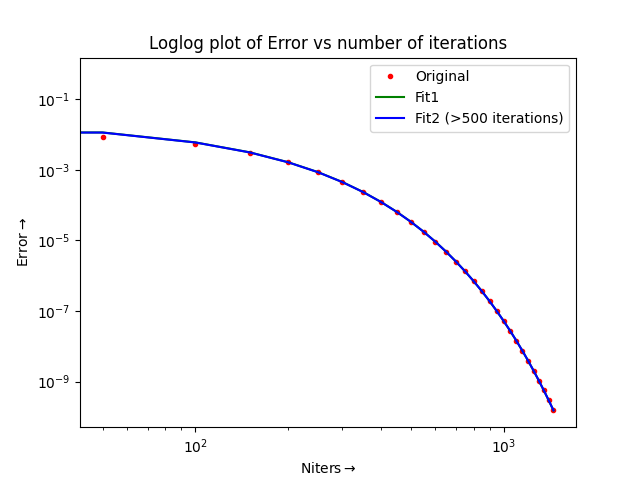
\includegraphics[scale=0.6]{plots/Loglog plot of Error vs number of iterations.png}
\caption{Best Fit of error (Loglog plot)}
\label{fig:Best Fit of error (Loglog plot)}
\end{figure}

\subsection{Plotting Max Cumulative Error}
The error reduces pretty slowly and thus this way of solving the Laplace's Equation is one of the worst possible methods. 
We can see in the following graph of max error on loglog scale that it reduces very slowly.
\begin{lstlisting}

def max_error(A,B,N):
    ''' Finds an upper bound for the error ''' 
    return -A*(np.exp(B*(N+0.5)))/B

\end{lstlisting}

\begin{figure}[h!]
    \centering
    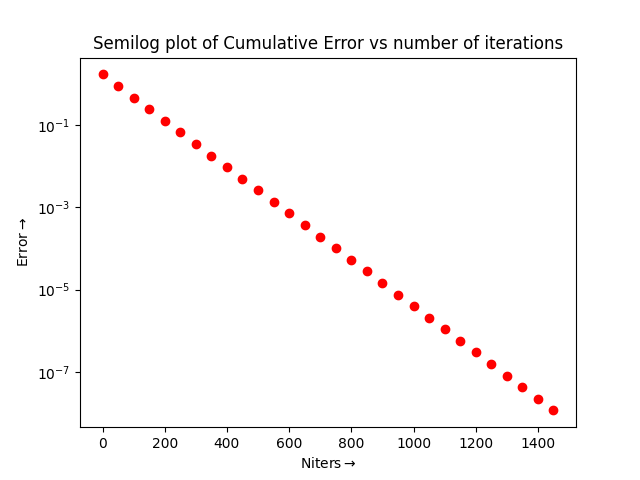
\includegraphics[scale=0.6]{plots/Semilog plot of Cumulative Error vs number of iterations.png}
    \caption{Cumulative error values on a log log scale}
    \end{figure}

\subsection{Stopping Criteria}
We notice that even though error is very small of the order of $1e-5$ it can be misleading as
what matters is the time required to decay by 1 time constant, which is large. One can even
that it decays very slowly after 500 iterations.

We calculate the cumulative error and show that even though error is decreasing at a steady
rate yet the cumulative error is large hence this method is not a good way to approximate
solving the laplace equation.


\section{Calculating Voltage at different regions on the plate}

The potential at any point on the plane is just the average of its neighbours, we keep iterating this process till the solution converges for
a given threshold. But we maintain the boundary conditions, that the side of the plate which
is grounded must remain 0 all the time and the voltage  for the surface in contact with the
wire is 1. Also note on boundarie,s the current needs to be tangential hence the gradient $\phi$ 
needs to be tangential. Thetfore the normal components of $\phi$ should be zero on the edges

\paragraph{3D Plot of Potential}
After finding the final potential values as mentioned previously we plot the surface potential as a 3D
plot with the potential value on the z axis. 


\begin{lstlisting}
def threeD_plot(self,X,Y,phi,cmap=plt.get_cmap('jet')):
    axes=p3.Axes3D(self.fig) 
    surf = axes.plot_surface(Y, X, phi.T, rstride=1, cstride=1,cmap=cmap)
    self.fig.colorbar(surf,shri$n_{k}$=0.5,pad=0.08)
    axes.set_zlabel(self.zlabel,fontsize=15) 
    self.general_funcs(axes)
\end{lstlisting}

\begin{figure}[ht!]
\centering
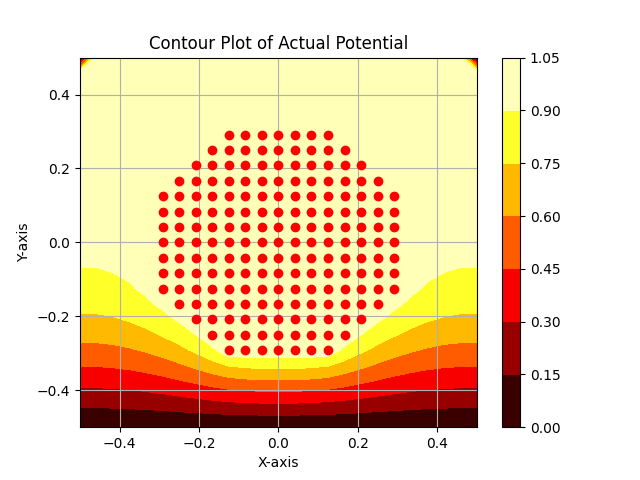
\includegraphics[scale=0.6]{plots/Contour Plot of Actual Potential.png}
\caption{2D Plot of Final Potential}
\label{fig:2D Plot of Potential}
\end{figure}


\begin{figure}[ht!]
\centering
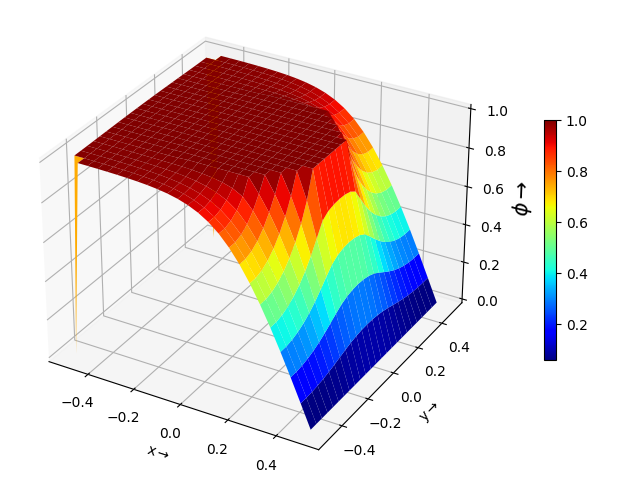
\includegraphics[scale=0.6]{plots/The 3-D surface plot of the potential.png}
\caption{3D Plot of Final Potential}
\label{fig:3D Plot of Potential}
\end{figure}

\newpage
\section{Calculating and Plotting Current Density}
The equations for current density in terms of potential is,
\begin{equation}
    J_x = -\partial\phi/\partial x
\end{equation}
\begin{equation}
    J_y = -\partial\phi/\partial y
\end{equation}
Here again we have to convert the differential equations to discrete domain. Thus,
\begin{equation}
    J_{x,ij} = 0.5*(\phi_{i,j-1} - \phi_{i,j+1})
\end{equation}
\begin{equation}
    J_{y,ij} = 0.5*(\phi_{i-1,j} - \phi_{i+1,j})
\end{equation}
\begin{lstlisting}

def solve_currents(phi,Nx,Ny):
    '''
    Function computes the current vectors ie: Jx , Jy
    '''
    Jx = np.zeros((Ny,Nx))
    Jy = np.zeros((Ny,Nx))
    Jx[:,1:-1] = 0.5*(phi[:,0:-2]-phi[:,2:])
    Jy[1:-1,:] = 0.5*(phi[2:, :]-phi[0:-2,:])

    return Jx,Jy

def quiver_plots(self,X,Y,Jx,Jy,wire_loc):
    axes=self.fig.add_subplot(111)
    axes.quiver(Y,X[::-1],Jx,Jy, scale = 5)
    axes.plot(X[:,0][wire_loc[0]],Y[0,:][wire_loc[1]],'ro')
    self.general_funcs(axes)

\end{lstlisting}
\begin{figure}[ht!]
\centering
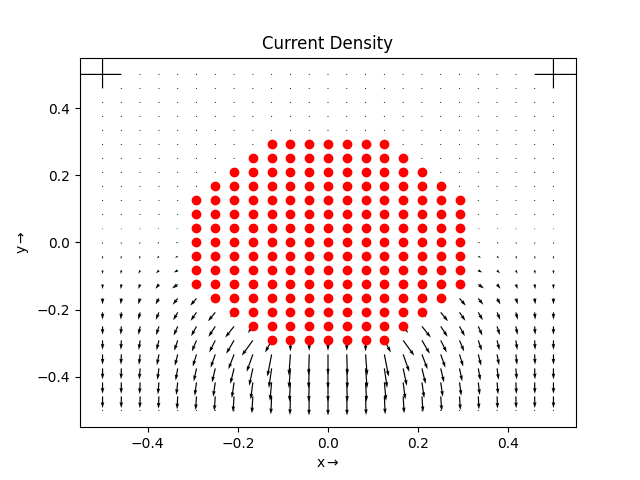
\includegraphics[scale=0.6]{plots/Current Density.png}
\caption{Vector plot of current flow}
\label{Vector plot of current flow}
\end{figure}

From the current density plot, we notice that hardly any current flows through the top part
of the wire. We observe that as the lower surface is grounded and the easiest way for current
to flow would be directly through the lower half plane. Thus all current vectors are located in
the lower half (half with the grounded side) and thus avoid they longer more resistive path.


\section{Finding temperature at different regions on the plate}

Having understood how currents flow in the plate we now study the heating pattern.As the
primary cause of heating is ohmic loss we expect to see a majority of heating happening where
currents are present. To find out Temperaure variation we solve the following equation using
the same Laplace approximation as done before.

\begin{equation}
    \nabla^2 T = -\frac{q}{\kappa} = -\frac{|J|^2}{\sigma \kappa}
\end{equation}
From the temperature plot and quiver plot we see that our intuition was correct and the majority of heating happens
where current are flowing
\begin{lstlisting}

def solve_temp(Ny,Nx,Jx,Jy,iters,wire_loc):
    '''
    Function computes the temperature vectors
    '''
    T=300*np.ones((Ny,Nx))
    for i in range(iters    ):
        T[1:-1,1:-1]=0.25*(T[1:-1,0:-2]+ T[1:-1,2:]+ T[0:-2,1:-1] + T[2:,1:-1]+(Jx[1:-1,1:-1])**2 +(Jy[1:-1,1:-1])**2)
        T[1:-1,0]=T[1:-1,1] # left boundary
        T[1:-1,-1]=T[1:-1,-2] # right boundary
        T[0,1:-1]=T[1,1:-1] # top boundary
        T[-1,1:-1] =300 # ground
        T[wire_loc]=300.0 #wire is at 300K
    return T

p9=General_Plotter(xlabel=r'x$\rightarrow$',ylabel=r'y$\rightarrow$',title='The 3-D surface plot of the Temperature',zlabel=r'$Temperature \rightarrow$')
p9.threeD_plot(X_coords,Y_coords, T)

\end{lstlisting}

\begin{figure}[ht!]
\centering
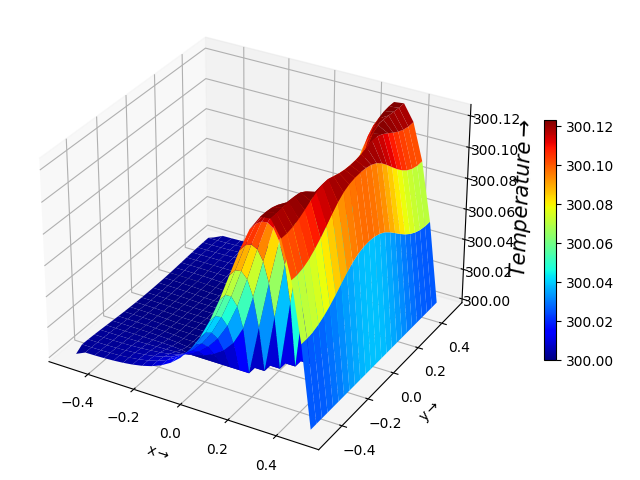
\includegraphics[scale=0.6]{plots/The 3-D surface plot of the Temperature.png}
\caption{Temperature Variation on the plate}
\label{fig:3d Plot of Potential}
\end{figure}


\newpage
\section{Conclusion}
Using a finite differentiation approximation , we find a solution to Laplace’s equation for a given
system. The error is seen to decay very slowly. Thus the chosen method of solving Laplace’s
equation is inefficient. On analysing the quiver plot of the currents , we notice that the current
was mostly restricted to the bottom of the wire and was perpendicular to the surface of the
electrode and the conductor. As a result heating effect is mostly seen on the lower half of the
plate.

\end{document}
